% ========================================
%	Header einbinden
% ========================================

\documentclass[bibtotoc,titlepage]{scrartcl}

% Deutsche Spracheinstellungen
\usepackage[ngerman,german]{babel, varioref}
\usepackage[T1]{fontenc}
\usepackage[utf8]{inputenc}

%\usepackage{marvosym}

\usepackage{amsfonts}
\usepackage{amssymb}
\usepackage{amsmath}
\usepackage{amscd}
\usepackage{amstext}
\usepackage{float}
\usepackage{caption}
\usepackage{wrapfig}
\usepackage{setspace}
\usepackage{threeparttable}
\usepackage{footnote}

\newfloat{formel}{htbp}{for}
\floatname{formel}{Formel}


\usepackage{longtable}

%\usepackage{bibgerm}

\usepackage{footnpag}

\usepackage{ifthen}                 %%% package for conditionals in TeX
\usepackage[amssymb]{SIunits}
%Fr textumflossene Bilder und Tablellen
%\usepackage{floatflt} - veraltet

%Fr Testzwecke aktivieren, zeigt labels und refs im Text an.
%\usepackage{showkeys}

% Abstand zwischen zwei Abs�zen nach DIN (1,5 Zeilen)
% \setlength{\parskip}{1.5ex plus0.5ex minus0.5ex}

% Einrckung am Anfang eines neuen Absatzes nach DIN (keine)
%\setlength{\parindent}{0pt}

% R�der definieren
% \setlength{\oddsidemargin}{0.3cm}
% \setlength{\textwidth}{15.6cm}

% bessere Bildunterschriften
%\usepackage[center]{caption2}


% Probleml�ungen beim Umgang mit Gleitumgebungen
\usepackage{float}

% Nummeriert bis zur Strukturstufe 3 (also <section>, <subsection> und <subsubsection>)
%\setcounter{secnumdepth}{3}

% Fhrt das Inhaltsverzeichnis bis zur Strukturstufe 3
%\setcounter{tocdepth}{3}

\usepackage{exscale}

\newenvironment{dsm} {\begin{displaymath}} {\end{displaymath}}
\newenvironment{vars} {\begin{center}\scriptsize} {\normalsize \end{center}}


\newcommand {\en} {\varepsilon_0}               % Epsilon-Null aus der Elektrodynamik
\newcommand {\lap} {\; \mathbf{\Delta}}         % Laplace-Operator
\newcommand {\R} { \mathbb{R} }                 % Menge der reellen Zahlen
\newcommand {\e} { \ \mathbf{e} }               % Eulersche Zahl
\renewcommand {\i} { \mathbf{i} }               % komplexe Zahl i
\newcommand {\N} { \mathbb{N} }                 % Menge der nat. Zahlen
\newcommand {\C} { \mathbb{C} }                 % Menge der kompl. Zahlen
\newcommand {\Z} { \mathbb{Z} }                 % Menge der kompl. Zahlen
\newcommand {\limi}[1]{\lim_{#1 \rightarrow \infty}} % Limes unendlich
\newcommand {\sumi}[1]{\sum_{#1=0}^\infty}
\newcommand {\rot} {\; \mathrm{rot} \,}         % Rotation
\newcommand {\grad} {\; \mathrm{grad} \,}       % Gradient
\newcommand {\dive} {\; \mathrm{div} \,}        % Divergenz
\newcommand {\dx} {\; \mathrm{d} }              % Differential d
\newcommand {\cotanh} {\; \mathrm{cotanh} \,}   %Cotangenshyperbolicus
\newcommand {\asinh} {\; \mathrm{areasinh} \,}  %Area-Sinus-Hyp.
\newcommand {\acosh} {\; \mathrm{areacosh} \,}  %Area-Cosinus-H.
\newcommand {\atanh} {\; \mathrm{areatanh} \,}  %Area Tangens-H.
\newcommand {\acoth} {\; \mathrm{areacoth} \,}  % Area-cotangens
\newcommand {\Sp} {\; \mathrm{Sp} \,}
\newcommand {\mbe} {\stackrel{\text{!}}{=}}     %Must Be Equal
\newcommand{\qed} { \hfill $\square$\\}
\renewcommand{\i} {\imath}
\def\captionsngerman{\def\figurename{\textbf{Abb.}}}

%%%%%%%%%%%%%%%%%%%%%%%%%%%%%%%%%%%%%%%%%%%%%%%%%%%%%%%%%%%%%%%%%%%%%%%%%%%%
% SWITCH FOR PDFLATEX or LATEX
%%%%%%%%%%%%%%%%%%%%%%%%%%%%%%%%%%%%%%%%%%%%%%%%%%%%%%%%%%%%%%%%%%%%%%%%%%%%
%%%
\ifx\pdfoutput\undefined %%%%%%%%%%%%%%%%%%%%%%%%%%%%%%%%%%%%%%%%% LATEX %%%
%%%
\usepackage[dvips]{graphicx}       %%% graphics for dvips
\DeclareGraphicsExtensions{.eps,.ps}   %%% standard extension for included graphics
\usepackage[ps2pdf]{thumbpdf}      %%% thumbnails for ps2pdf
\usepackage[ps2pdf,                %%% hyper-references for ps2pdf
bookmarks=true,%                   %%% generate bookmarks ...
bookmarksnumbered=true,%           %%% ... with numbers
hypertexnames=false,%              %%% needed for correct links to figures !!!
breaklinks=true,%                  %%% breaks lines, but links are very small
linkbordercolor={0 0 1},%          %%% blue frames around links
pdfborder={0 0 112.0}]{hyperref}%  %%% border-width of frames
%                                      will be multiplied with 0.009 by ps2pdf
%
\hypersetup{ pdfauthor   = {Hannes Franke; Julius Tilly},
pdftitle    = {V301 Innenwiderstand und Leistungsanpassung}, pdfsubject  = {Protokoll FP}, pdfkeywords = {V301, Innenwiderstand, Leistungsanpassung},
pdfcreator  = {LaTeX with hyperref package}, pdfproducer = {dvips
+ ps2pdf} }
%%%
\else %%%%%%%%%%%%%%%%%%%%%%%%%%%%%%%%%%%%%%%%%%%%%%%%%%%%%%%%%% PDFLATEX %%%
%%%
\usepackage[pdftex]{graphicx}      %%% graphics for pdfLaTeX
\DeclareGraphicsExtensions{.pdf}   %%% standard extension for included graphics
\usepackage[pdftex]{thumbpdf}      %%% thumbnails for pdflatex
\usepackage[pdftex,                %%% hyper-references for pdflatex
bookmarks=true,%                   %%% generate bookmarks ...
bookmarksnumbered=true,%           %%% ... with numbers
hypertexnames=false,%              %%% needed for correct links to figures !!!
breaklinks=true,%                  %%% break links if exceeding a single line
linkbordercolor={0 0 1},
linktocpage]{hyperref} %%% blue frames around links
%                                  %%% pdfborder={0 0 1} is the default
\hypersetup{
pdftitle    = {V301 Innenwiderstand und Leistungsanpassung}, 
pdfsubject  = {Protokoll AP}, 
pdfkeywords = {V301, Innenwiderstand, Leistungsanpassung},
pdfsubject  = {Protokoll AP},
pdfkeywords = {V301, Innenwiderstand, Leistungsanpassung}}
%                                  %%% pdfcreator, pdfproducer,
%                                      and CreationDate are automatically set
%                                      by pdflatex !!!
\pdfadjustspacing=1                %%% force LaTeX-like character spacing
\usepackage{epstopdf}
%
\fi %%%%%%%%%%%%%%%%%%%%%%%%%%%%%%%%%%%%%%%%%%%%%%%%%%% END OF CONDITION %%%
%%%%%%%%%%%%%%%%%%%%%%%%%%%%%%%%%%%%%%%%%%%%%%%%%%%%%%%%%%%%%%%%%%%%%%%%%%%%
% seitliche Tabellen und Abbildungen
%\usepackage{rotating}
\usepackage{ae}
\usepackage{
  array,
  booktabs,
  dcolumn
}
\makeatletter 
  \renewenvironment{figure}[1][] {% 
    \ifthenelse{\equal{#1}{}}{% 
      \@float{figure} 
    }{% 
      \@float{figure}[#1]% 
    }% 
    \centering 
  }{% 
    \end@float 
  } 
  \makeatother 


  \makeatletter 
  \renewenvironment{table}[1][] {% 
    \ifthenelse{\equal{#1}{}}{% 
      \@float{table} 
    }{% 
      \@float{table}[#1]% 
    }% 
    \centering 
  }{% 
    \end@float 
  } 
  \makeatother 
%\usepackage{listings}
%\lstloadlanguages{[Visual]Basic}
%\allowdisplaybreaks[1]
%\usepackage{hycap}
%\usepackage{fancyunits}

% ========================================
%	Angaben für das Titelblatt
% ========================================

\title{Versuch 61 - Der HeNe-LASER\\				% Titel des Versuchs 
\large TU Dortmund, Fakultät Physik\\ 
\normalsize Fortgeschrittenen-Praktikum}

\author{Jan Adam\\			% Name Praktikumspartner A
{\small \href{jan.adam@tu-dortmund.de}{jan.adam@tu-dortmund.de}}	% Erzeugt interaktiven einen Link
\and						% um einen weiteren Author hinzuzfügen
Dimitrios Skodras\\					% Name Praktikumspartner B
{\small \href{dimitrios.skodras@tu-dortmund.de}{dimitrios.skodras@tu-dortmund.de}}		% Erzeugt interaktiven einen Link
}
\date{21. Februar 2014}				% Das Datum der Versuchsdurchführung

% ========================================
%	Das Dokument beginnt
% ========================================

\begin{document}

% ========================================
%	Titelblatt erzeugen
% ========================================

\maketitle					% Jetzt wird die Titelseite erzeugt
\thispagestyle{empty} 				% Weder Kopfzeile noch Fußzeile

% ========================================
%	Der Vorspann
% ========================================

%\newpage					% Wenn Verzeichnisse auf einer neuen Seite beginnen sollen
%\pagestyle{empty}				% Weder Kopf- noch Fußzeile für Verzeichnisse

\tableofcontents

%\newpage					% eine neue Seite
%\thispagestyle{empty}				% Weder Kopf- noch Fußzeile für Verzeichnisse
%\listoffigures					% Abbildungsverzeichnis

%\newpage					% eine neue Seite
%\thispagestyle{empty}				% Weder Kopf- noch Fußzeile für Verzeichnisse
%\listoftables					% Tabellenverzeichnis
\newpage					% eine neue Seite


% ========================================
%	Kapitel
% ========================================

%\section{Einleitung}				% Bei Bedarf

\section{Theorie}
\setcounter{page}{1}
Ein LASER verstärkt kohärentes Licht einer bestimmten Wellenlänge, das durch angeregte Emission erzeugt und 
verstärkt wird (\textbf{L}ight \textbf{A}mplification by \textbf{S}timulated \textbf{E}mission of \textbf{R}adiation). Er besteht
dabei aus drei notwendigen Komponenten. Das aktive Lasermedium zur Bestimmung des Strahlungsspektrums und die Pumpquelle 
für die stimulierte Emission, sowie ein Resonator zur Verstärkung des Strahls.


\subsection{Absorbtion und Emission}
Grundsätzlich wird versucht, einfallendes Licht bei Wechselwirkung des Strahlungsfelds $\rho(\nu)$ mit dem Lasermedium zu verstärken. 
Vorzustellen ist sich ein System aus zwei möglichen Zuständen - Grundzustand und 1. angeregter Zustand - mit den zugehörigen 
Besetzungszahlen $n_1$ und $n_2$, sowie einer Energiedifferenz $\Delta E$. Das Zwei-Niveau-System ist zwar für die LASER-Konstruktion unzureichend,
soll hier jedoch zur Anschauung genügen.

Wenn nun ein Photon eine $\Delta E$ entsprechende Energie hat, kann es vom Medium absorbiert werden und das Atom anregen. 
Angeregte Atome können durch spontane Emission wiederum ein Photon jener Energie emittieren. Alternativ dazu ist es möglich,
dass mittels eines einfallenden Photons das Atom unter stimulierter Emission in den Grundzustand übergeht. Das hierbei
emittierte Photon ist in Energie, Phase und Ausbreitungsrichtung dem stimulierenden identisch. 
\begin{figure}[H]
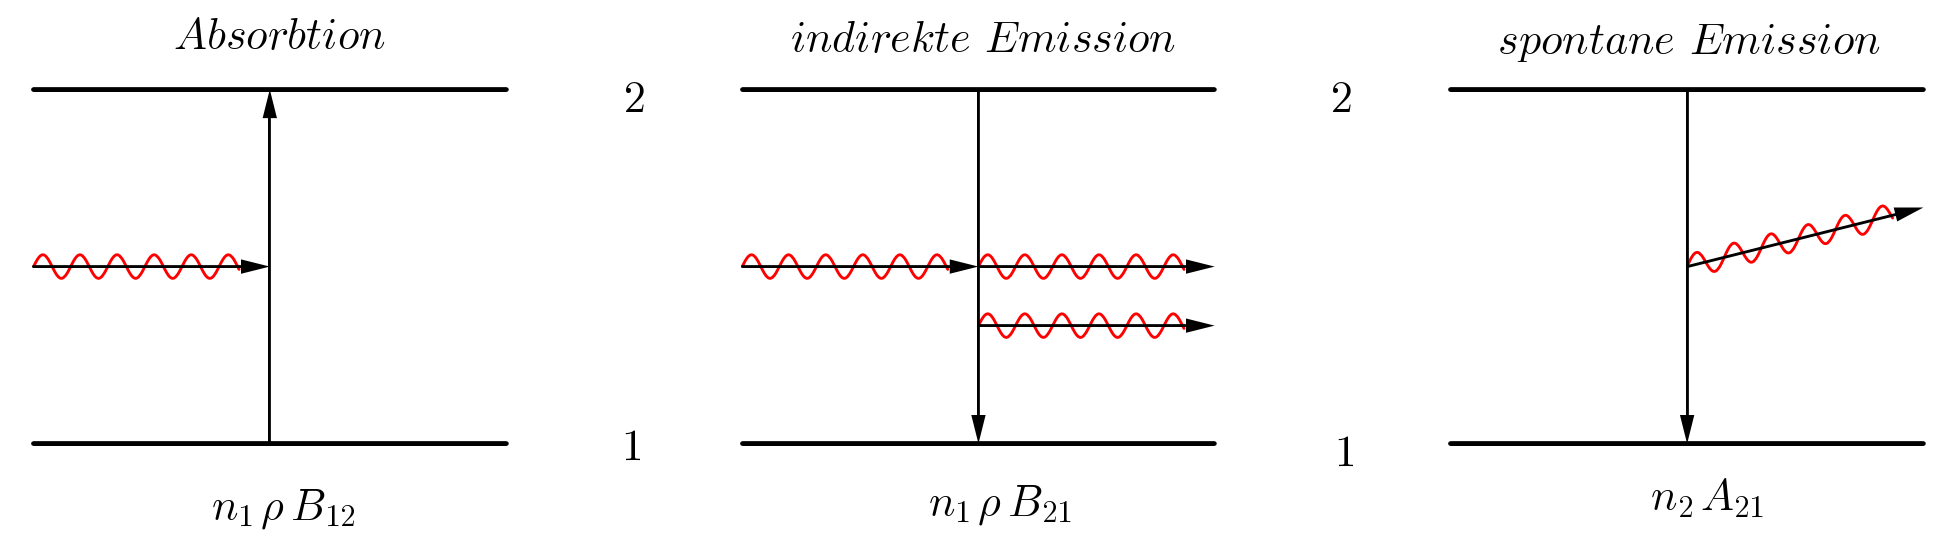
\includegraphics[width=\textwidth]{../pics/AbsEmi.png}
\caption{Absorbtion und Emission eines Zwei-Niveau-Systems}
\label{pic_AbsEmi}
\end{figure}
Die in Abbildung \ref{pic_AbsEmi} aufgeführten Ausdrücke stehen jeweils für die absorbierten bzw. emittierten Photonen $\dot N$,
bestimmt durch die Besetzungszahlen, das Strahlungsfeld und den nun hinzugekommenen konstanten Einsteinkoeffizienten $B_{12}, B_{21}$ und $A_{21}$, 
die jeweils als ein Maß der Übergangswahrscheinlichkeit zwischen den Niveaus 1 und 2 angesehen werden können. Sofern keine Verluste auftreten, lassen
sich zeitlichen Änderungen der Besetzungsdichten wie folgt formulieren
\begin{align*}
  \frac{\dx n_1}{\dx t} = -n_1\, B_{12}\, \rho + n_2\, B_{21} \rho + n_2\, A_{21}\\
  \frac{\dx n_2}{\dx t} = +n_1\, B_{12}\, \rho - n_2\, B_{21} \rho - n_2\, A_{21}
\end{align*}
Um die Kohärenz und die stete Verstärkung des Felds $\rho$ zu gewährleisten, ist ein Überwiegen von stimulierter Emission gegenüber spontaner Emission
erforderlich. Hierfür muss die Besetzungszahl des angeregten Zustands $n_2$ höher sein als die, des Grundzustands (Besetzungsinversion), was im thermischen Gleichgewicht
nicht mit der Maxwell-Boltzmann-Verteilung vereinbar ist. Daher muss dem LASER-Medium permanent Energie in Form von Elektronenstößen oder optischen
Anregungen zugeführt werden. 


\subsection{Aufbau des LASER}
Da die Verstärkung exponenziell mit dem Laufweg durchs LASER-Medium anwächst, ist es von hohem Interesse, diesen zu vergrößern. Dies geschieht durch
einen Resonator, der den Strahl mithilfe von zwei Spiegeln entsprechend Abbildung \ref{pic_Res} immer wieder durch das Medium führt. Beide Spiegel
können hierbei jeweils planparallel oder sphärisch sein. 
\begin{figure}[H]
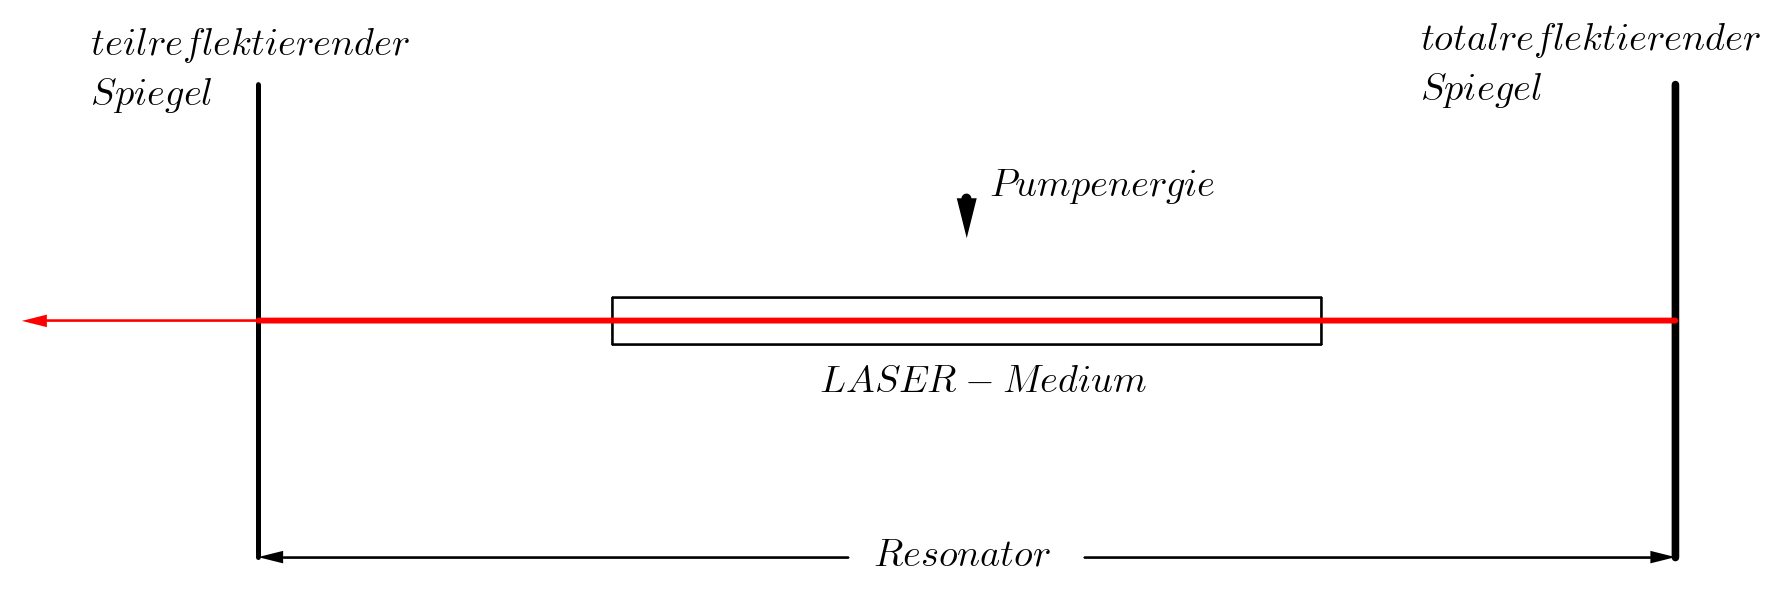
\includegraphics[width=\textwidth]{../pics/Res.png}
\caption{Konzeptioneller Aufbau eines LASERs}
\label{pic_Res}
\end{figure}
Bei einem konfokalen Resonator, dessen Spiegelbrennpunkte aufeinander fallen, sind die
unvermeidbaren formabhängigen Intensitätsverluste an den Spiegeln möglichst gering. Sind sie kleiner als die Verstärkung, so hat man einen selbsterregenden Oszillator
und damit einen optisch stabilen Resonator. Hierfür notwendig ist die Einhaltung des Bereichs \eqref{eq_ResBedingung} der Resonatorparameter $g_i = 1- \frac{L}{r_i}$, mit $L$ 
als Resonatorlänge und $r_i$ als Krümmungsradien der Spiegel.
\begin{align}
 0 \le g_1 \cdot g_2 < 1
 \label{eq_ResBedingung}
\end{align}
Der HeNe-LASER funktioniert mit einem Gasgemisch aus Helium und Neon im Verhältnis von 5 zu 1 bei einem Druck von etwa 133 Pa. Das Neon ist das 
LASER-Material und Helium wird Pumpgas benutzt. Die Besetzungsinversion wird durch elektrische Entladung realisiert, wobei das Helium in
metastabile Zustände angeregt wird. Diese Anregungsenergie wird durch STöße zweiter Art an das Neon übertragen, woraufhin Inversion auftritt. 
Ein Brewsterfenster ermöglicht einen verlustarmen Lichtaustritt. LASER-Aktivität wird bei mehreren Wellenlängen festgestellt, mit der roten $\lambda = 632,8$ nm
als intensivste.

\subsection{Eigenschwingungen des Resonators}
Die Resonanzbedingung \eqref{eq_ResBedingung} können wegen $L \gg \lambda_{\text{LASER}}$ viele Wellenlängen erfüllen. Die Anzahl $q$ der Wellenlängen
wird longitudinale Mode genannt. Transversale Moden sind durch Imperfektionen ebenfalls möglich und werden angelehnt an Hohlleitern mit TEM${_lpq}$ 
bezeichnet, mit $l$ und $p$ als transversale Modenzahlen und Knoten der x- bzw. y-Richtung. Aufgrund von zunehmenden Verlusten bei höheren Moden mit
geringerer Symmetrie, können nur wenige transversale Moden isoliert und verstärkt werden. Die Feldverteilungen für konfokale Resonatoren mit runden
Spiegeln werden angenähert durch
\begin{align*}
 E_{lpq} \propto& \cos(l \varphi) \frac{4\rho^2}{(1+Z^2)^(1+l)/2}L_p^q\left(\frac{4\rho^2}{1+Z^2} \right) \exp \left(-\frac{\rho^2}{1+Z^2} \right)\\
 &\exp \left(-i\left(\frac{(1+Z)\pi R}{\lambda} + \frac{\rho^2Z}{1+Z^2} - (l-2p+1)\left(\frac{\pi}{2}-\arctan \left(\frac{1-Z}{1+Z}\right)\right)\right)\right)\\ 
 &\hspace{6cm} \text{mit: } \rho = \left(\frac{2\pi}{\lambda R}\right)^\frac12\hspace{0.5 cm} \text{ und }\hspace{0.5 cm} Z = \frac{2z}{R}
\end{align*}
mit $L_p^q(x)$, denzugeordnete Laguerre-Polynomen. Hierdurch lassen sich beobachtbare Intensitätsverteilungen berechnen. Die verlustärmste Mode höchtster
Symmetrie ist die TEM$_{00}$ Grundmode ohne Nullstellen in transversaler Richtung. Beschrieben wird sie durch die Gaußverteilung
\begin{equation}
 I(r) = I_0 \e^{-2\frac{r^2}{w^2}},
\end{equation}
mit $I_0$ als Maximalintensität, $r$ als Abstand zur optischen Achse und 2$w$ als doppelten Strahlradius. Berechnen lässt sich der Strahlradius im
Abstand $z$ von der minimalen Taille $w_0$ durch
\begin{equation}
 w(z) = w_0 \sqrt{1+\left(\frac{\theta z}{w_0}\right)^2}, \hspace{1cm} \text{mit der Strahldivergenz } \theta = \frac{\lambda}{\pi}w_0. 
\end{equation}

\section{Durchführung}
Zur Justage des HeNe-LASERs befindet sich ein Justier-LASER auf einer optischen Schiene. Zudem können zwei Schirme mit Fadenkreuz und Beugungsblende
hinter den Justier-LASER und ans andere Ende der optischen Schine angebracht werden. Sind entsehende Beugungsringe direkt im Fadenkreuz, ist der 
LASER auf die optische Achse justiert. Nun werden Plasmarohr und Resonatorspiegel auf die optische Schiene gebracht und der Justier-LASER ausgestellt.
Nach Anstellen des Stroms auf $I$ = 6,5 mA und etwas Nachjustage ist eine LASER-Tätigkeit zu beobachten. 

Zur Überprüfung der Stabilitätsbedingung \eqref{eq_ResBedingung} wird die LASER-Leistung mithilfe einer Photodiode und die Resonatorlänge auf ihr Maximum eingestellt. Die 
Resonatorspiegel werden dabei stetig voneinander entfernt. Um TEM-Moden zu beobachten wird ein Wolframdraht ($d$ = 5 $\mu$m) zwischen Resonatorspiegel und LASER-Rohr angebracht und verschoben, sodass verschiedene
Moden auf dem optischen Schirm erkennbar sind. Sobald die Moden stabilisiert sind wird der Schirm durch eine Photodiode getauscht und die Intensität 
entlang des Strahlquerschnitts indirekt durch die Stromstärke gemessen.Die Polarisation lässt sich durch Einstellen eines Polarisators hinter dem teildurchlässigen Spiegel bestimmen. Hierzu wird die Intensität abermals mit
der Photodiode ermittelt in Abhängigkeit der Polarisationsrichtung. Die Wellenlänge lässt sich einfach durch den Abstand von Beugungsmaxima erzeugt
durch ein Gitter bzw. einen Spalt berechnen.
\section{Auswertung}
\subsection{Stabilitätsbedingungen}
Zunächst werden die Stabilitätsbedingungen überprüft. Folgenden Tabellen können die Aufgenommenen Wertepaare (Abstand/Stromstärke) entnommen werden, wobei die Werte aus Tabelle \ref{tab_kk} bei einem Aufbau mit zwei Konkavspiegeln und die Werte aus Tabelle \ref{tab_kf} mit einem Konkav- und einem Planspiegel aufgenommen wurden.
\begin{table}[htbp]
	% minipage mit (Blind-)Text
	\begin{minipage}[t]{0.45\textwidth} 
	\begin{tabular}[t]{c|c}
	cm & nA\\ \hline
	50,4 &   32,0\\
 	72    &  30,0\\
 	79     & 32,0\\
 	85      &33,0\\
 	90      &31,0\\
 	96      &30,0\\
 	101     &27,0\\
 	112     &13,0\\
 	123     &13,0\\
 	137     &21,0\\
 	143     &6,0\\
 	151     &4,7\\
 	155     &5,7\\
 	159     &6,2\\
 	166     &4,2\\
 	173     &2,0\\
 	176     &1,0
	\end{tabular}
	\caption{Messwerte konkav-konkav}
	\label{tab_kk}
	\end{minipage}
	\begin{minipage}[t]{0.45\textwidth} 
	\begin{tabular}[t]{c|c}
	cm & nA\\ \hline
	44,0&    26,0\\
	53,0&    13,0\\
	55,0&    16,0\\
	57,0&    7,9\\
	57,5&    4,5\\
	59,5&    3,5\\
	63,0&    4,0
	\end{tabular}
	\caption{Messwerte konkav-flach}
	\label{tab_kf}
	\end{minipage}
\end{table}

Eingetragen in ein Diagramm ergibt sich folgendes Bild:
\begin{figure}[h!]
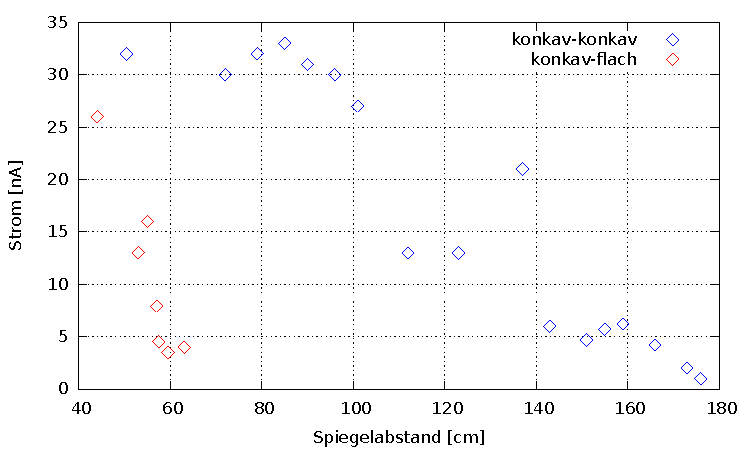
\includegraphics[scale=1]{../gnu/Abstand.pdf}
\caption{Beide Messreihen in ein Diagramm eingetragen}
\label{gra_abstand}
\end{figure}

Wie deutlich zu erkennen ist, lässt sich der Laserstrahl bei zwei konkaven Spiegeln deutlich länger aufrecht erhalten, als bei einem konkaven und einem flachen. Als Referenz dazu die theoretisch berechneten Stabilitätsbedingungen entsprechend Gleichung \eqref{eq_ResBedingung}:
\begin{figure}[h!]
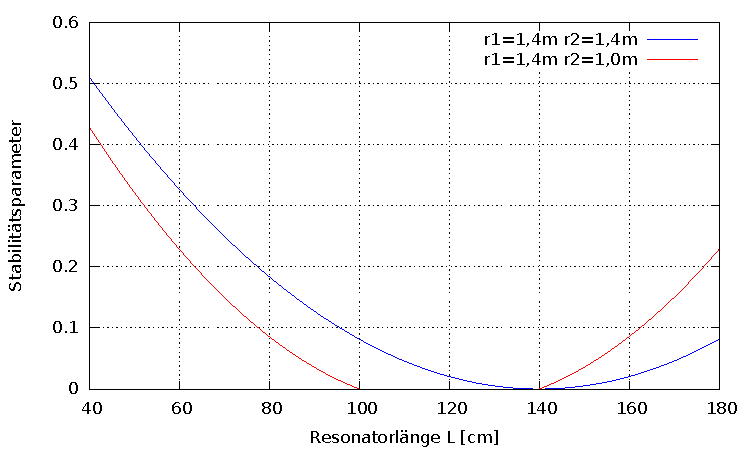
\includegraphics[scale=1]{../gnu/stabilitaetsparameter.pdf}
\caption{Theoretische Stabilitätbedingungen}
\label{gra_stabil}
\end{figure}

\parskip 340pt
\Large{Literatur}\\\\

% ========================================
%	Literaturverzeichnis
% ========================================

%\bibliographystyle{plainnat}			% Bibliographie-Style auswählen
%\bibliography{BIBDATEI}			% Literaturverzeichnis

% ========================================
%	Das Dokument endent
% ========================================

\end{document}
